%%%%%%%%%%%%%%%%%%%%%%%%%%%%%%%%%%%%%
% Document properties and packages
%%%%%%%%%%%%%%%%%%%%%%%%%%%%%%%%%%%%%
\documentclass[a4paper,12pt,final]{memoir}
\usepackage{CJKutf8}%中文支持

% misc
\renewcommand{\familydefault}{bch}	% font
\pagestyle{empty}					% no pagenumbering
\setlength{\parindent}{0pt}			% no paragraph indentation
% required packages (add your own)
\usepackage{flowfram}% column layou
\usepackage{marvosym}
\usepackage{textcomp}

\usepackage[top=1cm,left=1cm,right=1cm,bottom=1cm]{geometry}% margins
\usepackage{graphicx}										% figures
\usepackage{hyperref}
\definecolor{linkcolour}{rgb}{0,0.2,0.6}  %蓝色
\hypersetup{colorlinks,breaklinks,urlcolor=linkcolour, linkcolor=linkcolour}										% URLs
\usepackage[usenames,dvipsnames]{xcolor}					% color
\usepackage{multicol}										% columns env.
	\setlength{\multicolsep}{0pt}
\usepackage{paralist}										% compact lists
\usepackage{tikz}

%%%%%%%%%%%%%%%%%%%%%%%%%%%%%%%%%%%%%
% Create column layout
%%%%%%%%%%%%%%%%%%%%%%%%%%%%%%%%%%%%%
% define length commands
\setlength{\vcolumnsep}{\baselineskip}
\setlength{\columnsep}{\vcolumnsep}
%定义主题颜色,可选颜色 Maroon,ForestGreen,DarkOrchid,RoyalBlue,Turquoise,Cyan,etc,更多颜色参考xcolor包的颜色定义
\newcommand{\myThemeColor}{RoyalBlue}
% frame setup (flowfram package)
% left frame
\newflowframe{0.23\textwidth}{\textheight}{0pt}{0pt}[left]
	\newlength{\LeftMainSep}
	\setlength{\LeftMainSep}{0.23\textwidth}
	\addtolength{\LeftMainSep}{1\columnsep}
 
% small static frame for the vertical line
\newstaticframe{1.5pt}{\textheight}{\LeftMainSep}{0pt}
 
% content of the static frame
\begin{staticcontents}{1} %绘制分割线,使用tikz包绘制。如需改变风格线样式,请参考tikz教程,对于新手,不建议修改。
\hfill
\tikz{%
	\draw[loosely dotted,color=\myThemeColor,line width=1.5pt,yshift=0]
	(0,0) -- (0,\textheight);}%
\hfill\mbox{}
\end{staticcontents}
 
% right frame
\addtolength{\LeftMainSep}{1.5pt}
\addtolength{\LeftMainSep}{1\columnsep}
\newflowframe{0.7\textwidth}{\textheight}{\LeftMainSep}{0pt}[main01]


%%%%%%%%%%%%%%%%%%%%%%%%%%%%%%%%%%%%%
% define macros (for convience)
%%%%%%%%%%%%%%%%%%%%%%%%%%%%%%%%%%%%%
\newcommand{\Sep}{\vspace{1em}}
\newcommand{\SmallSep}{\vspace{0.9em}}

\newenvironment{AboutMe}
	{\ignorespaces\textbf{\color{\myThemeColor} About me}}
	{\Sep\ignorespacesafterend}
%定义section	
\newcommand{\CVSection}[1]
	{\Large\textbf{#1}\par
	\vspace{0.2cm}\normalsize\normalfont}

\newcommand{\CVItem}[1]
	{\textbf{\color{\myThemeColor} #1}}


%%%%%%%%%%%%%%%%%%%%%%%%%%%%%%%%%%%%%
% Begin document
%%%%%%%%%%%%%%%%%%%%%%%%%%%%%%%%%%%%%
\begin{document}

\begin{CJK*}{UTF8}{gbsn}%选择字体,黑体
% Left frame 左边内容在此定义
%%%%%%%%%%%%%%%%%%%%
\begin{figure}
	\hfill
	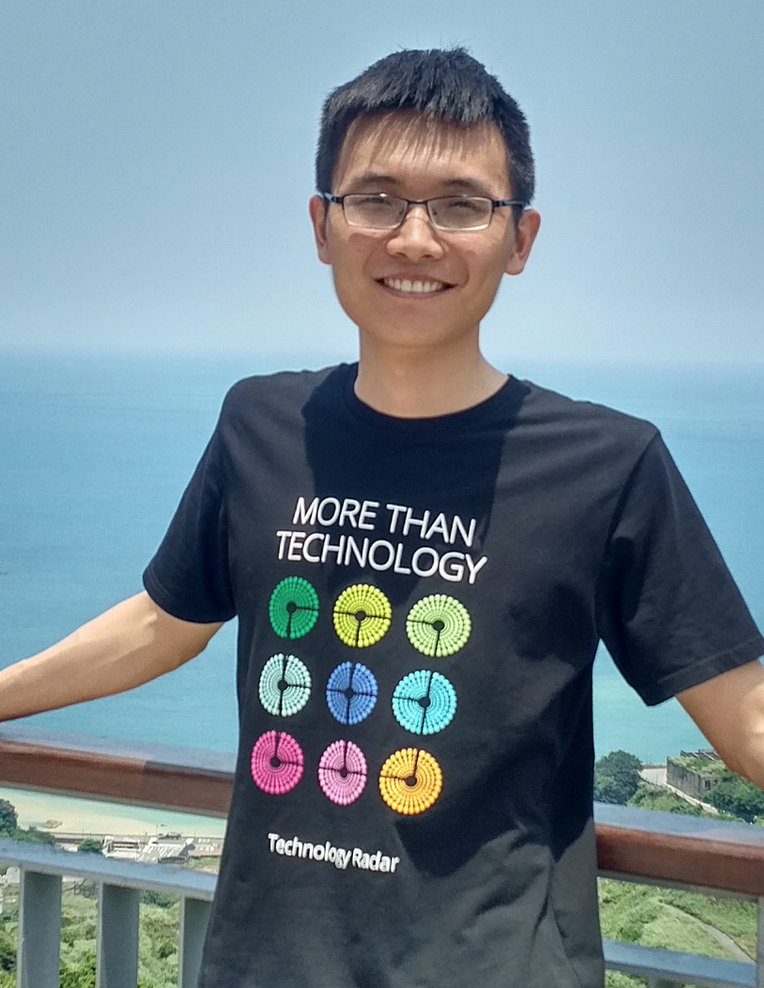
\includegraphics[width=0.7\columnwidth]{photo}
	\vspace{-7cm}
\end{figure}
\begin{flushright}\footnotesize
.\\
\vskip 6cm
    \raggedright
	\CVItem{{\large 个人信息:}}\\
	电子邮件:\\
	\href{mailto:lc1990linux@gmail.com}{lc1990linux@gmail.com}  \\
	个人主页:\\
	\href{http://linchen2chris.github.io/}{linchen2chris.github.io} \\
	手机:\\ 13540394019	
  
	\CVItem{{\large 语言能力:}}\\
  \SmallSep
	\textit{\textbf{中文}:母语 \\\textbf{英语}:流利,可以和海外工程师合作\\}
	
	%% \SmallSep
	%% \textit{能够在Android和WP平台上编写简单的Apps,熟练使用\LaTeX 和LINUX}
	
	%% \CVItem{{\large 爱好:}}\\
	%% \textit{长跑,旅游,摄影,健身,吉他}
	%% \SmallSep
\end{flushright}\normalsize
\framebreak


% Right frame 右边内容在此定义
%%%%%%%%%%%%%%%%%%%%
\Huge\bfseries {\color{\myThemeColor} 林~~晨}\\
\normalsize\normalfont

% Education
\CVSection{教育背景}
\hrule
\SmallSep
\CVItem{2011 - 2014\hfill\textsc{四川大学}}\\
\textit{-计算机学院}\\
\textit{-理学硕士学位}
\\
\CVItem{2007 - 2011\hfill\textsc{四川大学}}\\
\textit{-公共管理学院}\\
\textit{-管理学学士学位}\\
\\
%% Skills
\CVSection{专业技能}
\hrule
\SmallSep
\CVItem{前端相关}\\
\textit{$\bullet$ 熟悉react, react-native, redux, alt框架,js/CSS/html, jss, typescript等} \\
\\
\CVItem{后端相关}\\
\textit{$\bullet$ 熟悉spring boot框架, nodejs, mongodb等 } \\
\\
\CVItem{其它}\\
\textit{$\bullet$ 熟悉CI/CD, Agile, Scrum,TDD等开发方法, 前后端测试框架 }\\
\\

% Experience
\CVSection{工作经历}
\hrule
\SmallSep
\CVItem{2016.10 - 至今 \hfill ThoughtWorks}\\
\textit{$\bullet$ 担任软件工程师,Tech Leader,为一家大型海外金融企业提供软件交付服务} \\
\textit{$\bullet$ 项目技术栈:后端采用Spring boot搭建微服务架构,前端采用~react~+~flux~} \\
\textit{$\bullet$ 项目采用成都-海外合作开发的形式,通过网页收集用户信息,验证用户,提交用户信息,在线申请保险,在线开
  通银行卡}\\
\textit{$\bullet$ 我承担了大部分前端工作和部分后端工作,搭建了可与其它组共用
  的~react~组件库; 承担了团队的技术管理工作,帮助多位后来的同事熟悉项目}\\
\\
\CVItem{2015.10 - 2016.10 \hfill 创业项目}\\
\textit{$\bullet$ 参加并主导创业项目。该项目旨在建立一个医院血透管理系统} \\
\textit{$\bullet$ 项目技术栈:后端采用nodejs + mongodb, 前端采用react+redux} \\
\textit{$\bullet$ 项目通过患者移动端,和医院~web~端协同工作,实现肾病患者的全周
  期管理。我承担了大部分后端api和数据库的开发工作,为所有的前端提供服务,也承担
  了部分前端页面的开发。}\\
\\
\CVItem{2014.07 - 2015.09\hfill CIeNET,瞬联科技}\\
\textit{$\bullet$ 担任后端工程师,开发并维护电信后台计费系统Kenan} \\
\textit{$\bullet$ 项目主要采用C/C++, 基于Unix服务器开发,熟悉vim, emacs, unix等
  开发工具和开发环境, 所在小组参与了实时计费系统和后计费系统的整合。} \\

% CAMPU
%% \CVSection{专业经历}
%% \hrule
%% \SmallSep
%% \CVItem{2012.04 - 2013.03, 大学生创新项目(IPP)\hfill\emph{研究员}}\\
%% \textit{$\bullet$ 主导参加IPP项目,研究并可视化激光等离子体在真空环境下的聚焦点。} 
%% \\
%% \CVItem{2013.05 - 2013.09, 大陆台湾能源合作\hfill\emph{研究专员}}\\
%% \textit{$\bullet$ 调研大陆能源供给和消费情况,相关资料提供给台湾学者使用,促进两岸科学交流} 
%% \\
%% \CVItem{2013.02 - 2013.10, 奥迪绿色能源竞赛\hfill\emph{团队领导}}\\
%% \textit{$\bullet$ 领头参加绿色能源竞赛,我们的作品是“智能绿色候车公交站台”,并获一等奖}
%% \\
%% \CVItem{2012.06 - 2012.09, 社会实践\hfill\emph{团队领导}}\\
%% \textit{$\bullet$ 组织16个人的社会实践团队,深入甘肃会宁,为一个公益福利网站调查并收集贫困家庭信息,该项目获上海市社会实践优秀项目} 

% HONORS & SCHOLARSHIPS
%% \CVSection{个人荣誉}
%% \hrule
%% \SmallSep
%% 	\begin{tabular}{l|l}
%% 		$\Rightarrow$ 2014.10&\textit{法国大使馆杰出人才奖学金}\footnotesize\\
%% 		$\Rightarrow$ 2013.10&\textit{奥迪绿色能源竞赛一等奖}\\
%% 		$\Rightarrow$ 2012.12&\textit{晨兴企业奖学金}\\
%% 		$\Rightarrow$ 2012.10&\textit{连续三年获得上海交大优秀学生奖学金}\\
%% 		$\Rightarrow$ 2011.04&\textit{上海市社会实践优秀项目}\footnotesize\\
%% 	\end{tabular}

%%%%%%%%%%%%%%%%%%%%%%%%%%%%%%%%%%%%%
% End document
%%%%%%%%%%%%%%%%%%%%%%%%%%%%%%%%%%%%%
\end{CJK*}
\end{document}
